% В этом документе преамбула

%%% Работа с русским языком
\usepackage{cmap}					% поиск в PDF
\usepackage{mathtext} 				% русские буквы в формулах
\usepackage[T2A]{fontenc}			% кодировка
\usepackage[utf8]{inputenc}			% кодировка исходного текста
\usepackage[english,russian]{babel}	% локализация и переносы
\usepackage{indentfirst}			% чтобы первый абзац в разделе отбивался красной строкой
\frenchspacing						% тонкая настройка пробелов

%%% Приведение начертания букв и знаков к русской типографской традиции
\renewcommand{\epsilon}{\ensuremath{\varepsilon}}
\renewcommand{\phi}{\ensuremath{\varphi}}			% буквы "эпсилон"
\renewcommand{\kappa}{\ensuremath{\varkappa}}		% буквы "каппа"
\renewcommand{\le}{\ensuremath{\leqslant}}			% знак меньше или равно
\renewcommand{\leq}{\ensuremath{\leqslant}}			% знак меньше или равно
\renewcommand{\ge}{\ensuremath{\geqslant}}			% знак больше или равно
\renewcommand{\geq}{\ensuremath{\geqslant}}			% знак больше или равно
\renewcommand{\emptyset}{\varnothing}				% знак пустого множества

%%% Дополнительная работа с математикой
\usepackage{amsmath,amsfonts,amssymb,amsthm,mathtools} % AMS
\usepackage{icomma} % "Умная" запятая: $0,2$ --- число, $0, 2$ --- перечисление

%% Номера формул
\mathtoolsset{showonlyrefs=true} % Показывать номера только у тех формул, на которые есть \eqref{} в тексте.

%% Свои команды

% операции, не определённые (или имеющие иные обохначения) в мат. пакетах
\DeclareMathOperator{\sgn}{\mathop{sgn}}				% ф-ия sgn
\renewcommand{\tg}{\mathop{\mathrm{tg}}\nolimits}		% обозначение тангенса

%% Перенос знаков в формулах (по Львовскому)
\newcommand*{\hm}[1]{#1\nobreak\discretionary{}
{\hbox{$\mathsurround=0pt #1$}}{}}

%%% Работа с картинками
\usepackage{graphicx}  % Для вставки рисунков
\graphicspath{{images/}{images2/}}  % папки с картинками
\setlength\fboxsep{3pt} % Отступ рамки \fbox{} от рисунка
\setlength\fboxrule{1pt} % Толщина линий рамки \fbox{}
\usepackage{wrapfig} % Обтекание рисунков текстом

%%% Работа с таблицами
\usepackage{array,tabularx,tabulary,booktabs} % Дополнительная работа с таблицами
\usepackage{longtable}  % Длинные таблицы
\usepackage{multirow} % Слияние строк в таблице

%%% Теоремы
\theoremstyle{plain} % Это стиль по умолчанию, его можно не переопределять.
\newtheorem{theorem}{Теорема}[section]
\newtheorem{lemma}{Лемма}[section]
\newtheorem{definition}[theorem]{Определение}
\newtheorem{property}{Свойство}
 
\theoremstyle{definition} % "Определение"
\newtheorem{corollary}{Следствие}[theorem]
\newtheorem{exmp}{Пример}[section]
 
\theoremstyle{remark} % "Примечание"
\newtheorem*{nonum}{Решение}
\newtheorem*{evidence}{Доказательство}
\newtheorem*{remark}{Примечание}

%%% Программирование
\usepackage{etoolbox} % логические операторы

%%% Страница
\usepackage{extsizes} % Возможность сделать 14-й шрифт
\usepackage{geometry} % Простой способ задавать поля
	\geometry{top=25mm}
	\geometry{bottom=35mm}
	\geometry{left=35mm}
	\geometry{right=20mm}

%\usepackage{fancyhdr} % Колонтитулы
% 	\pagestyle{fancy}
 	%\renewcommand{\headrulewidth}{0pt}  % Толщина линейки, отчеркивающей верхний колонтитул
% 	\lfoot{Нижний левый}
% 	\rfoot{Нижний правый}
% 	\rhead{Верхний правый}
% 	\chead{Верхний в центре}
% 	\lhead{Верхний левый}
%	\cfoot{Нижний в центре} % По умолчанию здесь номер страницы

\usepackage{setspace} % Интерлиньяж (межстрочные интервалы)
%\onehalfspacing % Интерлиньяж 1.5
%\doublespacing % Интерлиньяж 2
%\singlespacing % Интерлиньяж 1

\usepackage{lastpage} % Узнать, сколько всего страниц в документе.

\usepackage{soulutf8} % Модификаторы начертания

\usepackage{hyperref}
\usepackage[usenames,dvipsnames,svgnames,table,rgb]{xcolor}
\hypersetup{				% Гиперссылки
    unicode=true,           % русские буквы в раздела PDF
    pdftitle={Заголовок},   % Заголовок
    pdfauthor={Автор},      % Автор
    pdfsubject={Тема},      % Тема
    pdfcreator={Создатель}, % Создатель
    pdfproducer={Производитель}, % Производитель
    pdfkeywords={keyword1} {key2} {key3}, % Ключевые слова
    colorlinks=true,       	% false: ссылки в рамках; true: цветные ссылки
    linkcolor=MidnightBlue,          % внутренние ссылки
    citecolor=black,        % на библиографию
    filecolor=magenta,      % на файлы
    urlcolor=blue           % на URL
}

\usepackage{csquotes} % Еще инструменты для ссылок

%\usepackage[style=authoryear,maxcitenames=2,backend=biber,sorting=nty]{biblatex}

\usepackage{multicol} % Несколько колонок

%%% Работа с графикой
\usepackage{tikz}
\usetikzlibrary{calc}
\usepackage{tkz-euclide}
\usetikzlibrary{arrows}
\usepackage{pgfplots}
\usepackage{pgfplotstable}

%%% Настройка подписей к плавающим объектам
\usepackage{floatrow}	% размещение
\usepackage{caption}	% начертание
\captionsetup[figure]{labelfont=bf,textfont=it,font=footnotesize}	% нумерация и надпись курсивом
% для подфигур: заголовок подписи полужирный, текст заголовка обычный
% выравнивание является неровным (т.е. выровненным по левому краю)
% singlelinecheck = off означает, что настройка выравнивания используется, даже если заголовок имеет длину только одну строку.
% если singlelinecheck = on, то заголовок всегда центрируется, когда заголовок состоит только из одной строки.
\captionsetup[subfigure]{labelfont=bf,textfont=normalfont,singlelinecheck=off,justification=raggedright}

%%% Stuff для графиков и рисунков



\begin{document}

\textit{Почаев Никита Алексеевич, гр. 8381}

\section*{Формула полной вероятности. Формула Байеса. (ДЗ на 07.03.20)}

\subsection*{Задача 1.}

Белые и чёрные шары распределены по ящикам следующим образом:

\begin{figure}[H]
	\center{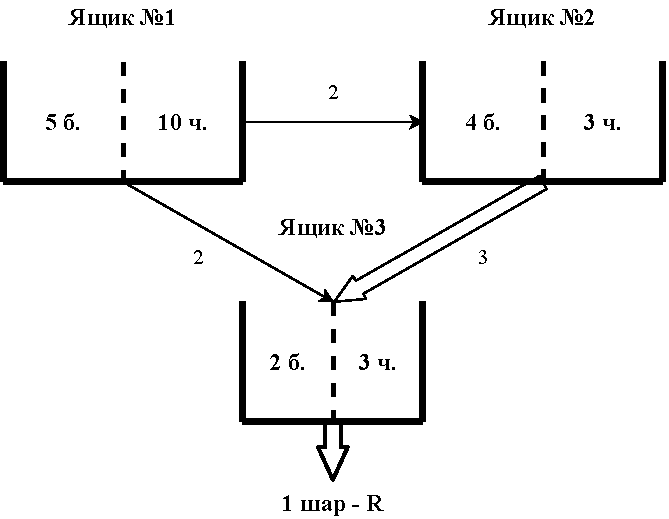
\includegraphics[scale=1]{./media/Homework-29-02-20_2.pdf}}
\end{figure}

а) Вытащен белый шар, определить вероятность, что в 1-м ящике осталось 5 белых.

\textit{Решение:}

События $A_i, 0 \le i \le 2$ - из 1-ого ящика в 3-ий переложили $i$ белых шаров образуют ПГС. Всего возможных вариантов данного действия: $C_{15}^2 = 105$.

События $B_j, 0 \le j \le 2$ - из 1-го ящика во 2-й переложили $j$ белых шаров.

Построим таблицу условных вероятностей для каждого $B_j$-ого. Всего вариантов данного события (учитывая, что два уже вытащены из 1-го ящика): $C_{13}^2 = 78$. Если, например, из 1-го ящика в 3-й переложили 1 белый, то в 1-м ящике осталось 4 белых и 9 черных.

\begin{table}[h]
	\centering\makegapedcells
	\begin{tabular}{|c|c|c|c|}
		\hline
		$i$          & 0                                                      & 1                                                       & 2                                                       \\ \hline
		$P(A_i)$     & $\frac{C_5^0 \cdot C_{10}^2}{C_{15}^2} = \frac{3}{7}$  & $\frac{C_5^1 \cdot C_{10}^1}{C_{15}^2} = \frac{10}{21}$ & $\frac{C_5^2 \cdot C_{10}^0}{C_{15}^2} = \frac{2}{21}$  \\ \hline
		$P(B_0|A_i)$ & $\frac{C_5^0 \cdot C_{8}^2}{C_{13}^2} = \frac{14}{39}$ & $\frac{C_4^0 \cdot C_{9}^2}{C_{13}^2} = \frac{6}{13}$   & $\frac{C_3^0 \cdot C_{10}^2}{C_{13}^2} = \frac{15}{26}$ \\ \hline
		$P(B_1|A_i)$ & $\frac{C_5^1 \cdot C_{8}^1}{C_{13}^2} = \frac{20}{39}$ & $\frac{C_4^1 \cdot C_{9}^1}{C_{13}^2} = \frac{6}{13}$   & $\frac{C_3^1 \cdot C_{10}^1}{C_{13}^2} = \frac{5}{13}$  \\ \hline
		$P(B_2|A_i)$ & $\frac{C_5^2 \cdot C_{8}^0}{C_{13}^2} = \frac{5}{39}$  & $\frac{C_4^2 \cdot C_{9}^0}{C_{13}^2} = \frac{1}{13}$   & $\frac{C_3^2 \cdot C_{10}^0}{C_{13}^2} = \frac{1}{26}$  \\ \hline
	\end{tabular}
\end{table}

По формуле ПГС найдём вероятности $P(B_0), P(B_1), P(B_2)$:

\[ P(B_0) = \sum_{i=0}^{2} P(B_0|A_i) \cdot P(A_i) = \dfrac{3}{7} \]
\[ P(B_1) = \sum_{i=0}^{2} P(B_1|A_i) \cdot P(A_i) = \dfrac{10}{21} \]
\[ P(B_2) = \sum_{i=0}^{2} P(B_2|A_i) \cdot P(A_i) = \dfrac{2}{21} \]

Видно, что вероятности $B_0, B_1, B_2$ также образуют ПГС.

События $C_k$ - из 2-го ящика в 3-й переложили $k$ белых шаров.

\begin{table}[h]
	\centering\makegapedcells
	\begin{tabular}{|c|c|c|c|}
		\hline
		$B_i$        & $B_0$                                             & $B_1$                                             & $B_2$                                             \\ \hline
		$P(B_i)$     & $\frac{3}{7}$                                     & $\frac{10}{21}$                                   & $\frac{2}{21}$                                    \\ \hline
		$P(C_0|B_i)$ & $\frac{C_4^0 \cdot C_5^3}{C_9^3} = \frac{5}{42}$  & $\frac{C_5^0 \cdot C_4^3}{C_9^3} = \frac{1}{21}$  & $\frac{C_6^0 \cdot C_3^3}{C_9^3} = \frac{1}{84}$  \\ \hline
		$P(C_1|B_i)$ & $\frac{C_4^1 \cdot C_5^2}{C_9^3} = \frac{10}{21}$ & $\frac{C_5^1 \cdot C_4^2}{C_9^3} = \frac{5}{14}$  & $\frac{C_6^1 \cdot C_3^2}{C_9^3} = \frac{3}{14}$  \\ \hline
		$P(C_2|B_i)$ & $\frac{C_4^2 \cdot C_5^1}{C_9^3} = \frac{5}{14}$  & $\frac{C_5^2 \cdot C_4^1}{C_9^3} = \frac{10}{21}$ & $\frac{C_6^2 \cdot C_3^1}{C_9^3} = \frac{15}{28}$ \\ \hline
		$P(C_3|B_i)$ & $\frac{C_4^3 \cdot C_5^0}{C_9^3} = \frac{1}{21}$  & $\frac{C_5^3 \cdot C_4^0}{C_9^3} = \frac{5}{42}$  & $\frac{C_6^3 \cdot C_3^0}{C_9^3} = \frac{5}{21}$  \\ \hline
	\end{tabular}
\end{table}

По формуле ПГС найдём вероятности $P(C_0), P(C_1), P(C_2), P(C_3)$:

\[ P(C_0) = \sum_{i=0}^{2} P(C_0|B_i) \cdot P(B_i) = \dfrac{11}{147} \]
\[ P(C_1) = \sum_{i=0}^{2} P(C_1|B_i) \cdot P(B_i) = \dfrac{58}{147} \]
\[ P(C_2) = \sum_{i=0}^{2} P(C_2|B_i) \cdot P(B_i) = \dfrac{190}{441} \]
\[ P(C_3) = \sum_{i=0}^{2} P(C_3|B_i) \cdot P(B_i) = \dfrac{44}{441} \]

\[ \sum_{i=0}^{3} P(C_i) = 1 \Rightarrow \text{ события образуют ПГС} \]

Событие $D_l$ – в 3-й ящик попало $l$ белых (из 1-го и 2-го ящика).

\begin{table}[h]
	\centering\makegapedcells
	\begin{tabular}{|c|c|c|c|c|c|c|}
		\hline
		$l$                & 0            & 1                                                                      & 2                                                                                        & 3                                                                                        & 4                                                                      & 5            \\ \hline
		Комбинация событий & $(C_0, A_0)$ & \begin{tabular}[c]{@{}c@{}}$(C_1, A_0)$\\ \\ $(C_0, A_1)$\end{tabular} & \begin{tabular}[c]{@{}c@{}}$(C_2, A_0)$\\ \\ $(C_1, A_1)$\\ \\ $(C_0, A_2)$\end{tabular} & \begin{tabular}[c]{@{}c@{}}$(C_3, A_0)$\\ \\ $(C_2, A_1)$\\ \\ $(C_1, A_2)$\end{tabular} & \begin{tabular}[c]{@{}c@{}}$(C_3, A_1)$\\ \\ $(C_2, A_2)$\end{tabular} & $(C_3, A_2)$ \\ \hline
	\end{tabular}
\end{table}

\[ P(D_0) = P(C_0) \cdot P(A_0) = 0.032 \]
\[ P(D_1) = P(C_1) \cdot P(A_0) + P(C_0) \cdot P(A_1) = 0.204 \]
\[ P(D_2) = P(C_2) \cdot P(A_0) + P(C_1) \cdot P(A_1) + P(C_0) \cdot P(A_2) = 0.379 \]
\[ P(D_3) = P(C_3) \cdot P(A_0) + P(C_2) \cdot P(A_1) + P(C_1) \cdot P(A_2) = 0.2855 \]
\[ P(D_4) = P(C_3) \cdot P(A_1) + P(C_2) \cdot P(A_2) = 0.0885 \]
\[ P(D_5) = P(C_3) \cdot P(A_2) = 0.0095 \]

\[ \sum_{i=0}^{5} P(D_i) \approx 1 \Rightarrow \text{ события образуют ПГС} \]

В результате в 3-ем ящике 10 шаров.

Событие $E$ - из 3-го ящика достали белый шар.

\begin{table}[h]
	\centering\makegapedcells
	\begin{tabular}{|c|c|c|c|c|c|c|}
		\hline
		$i$        & 0              & 1              & 2              & 3              & 4              & 5              \\ \hline
		$P(D_i)$   & 0.032          & 0.204          & 0.379          & 0.2855         & 0.0885         & 0.0095         \\ \hline
		$P(E|D_i)$ & $\frac{2}{10}$ & $\frac{3}{10}$ & $\frac{4}{10}$ & $\frac{5}{10}$ & $\frac{6}{10}$ & $\frac{7}{10}$ \\ \hline
	\end{tabular}
\end{table}

\[ P(E) = \sum_{i=0}^{5} P(D_i)P(E|D_i) = 0.4217 \]

Событие $F$ - в 1-ом ящике осталось 5 белых шаров, т.е. из него достали все чёрные, а белый шар, который достали из 3-его изначально был в нём или пришёл из 2-ого.

Должна выполниться совокупность событий $A_0$ - из 1-ого ящика во 3-ий ушло 0 белых шаров, $B_0$ - из 1-ого ящика во 2-ой ушло 0 белых шаров. В совокупности в 3-ий ящик может придти от 0 до 3-х шаров, что соотвествует событиям $D_0-D_3$. При этом нам необходима выполнимость указанных событий $A_0$ и $B_0$.

Подходящие комбинации для событий $D_l$:

\begin{table}[h]
	\centering\makegapedcells
	\begin{tabular}{|c|c|c|c|c|}
		\hline
		& 0            & 1            & 2            & 3            \\ \hline
		Комбинация событий & $(C_0, A_0)$ & $(C_1, A_0)$ & $(C_2, A_0)$ & $(C_3, A_0)$ \\ \hline
	\end{tabular}
\end{table}

Также учитываем, что для событий $C_k'$ мы рассматриваем случае, при которых выполняется $B_0$, т.е. используя таблицу, приведённую выше, получаем:

\[ P(C_0') = P(C_0B_0) = P(C_0|B_0)P(B_0) = \dfrac{5}{42} \cdot \dfrac{3}{7} = \dfrac{5}{98} \]
\[ P(C_1') = P(C_1B_0) = P(C_1|B_0)P(B_0) = \dfrac{10}{21} \cdot \dfrac{3}{7} = \dfrac{10}{49} \]
\[ P(C_2') = P(C_2B_0) = P(C_2|B_0)P(B_0) = \dfrac{5}{14} \cdot \dfrac{3}{7} = \dfrac{15}{98} \]
\[ P(C_3') = P(C_3B_0) = P(C_3|B_0)P(B_0) = \dfrac{1}{21} \cdot \dfrac{3}{7} = \dfrac{1}{49} \]

Тогда:

\[ P(D_0') = P(D_0C_0B_0) = P(C_0') \cdot P(A_0) = P(C_0B_0) \cdot P(A_0) = \dfrac{15}{686} \]
\[ P(D_1') = P(D_1C_1B_0) = P(C_1') \cdot P(A_0) = \dfrac{30}{343} \]
\[ P(D_2') = P(D_2C_2B_0) = P(C_2') \cdot P(A_0) = \dfrac{45}{686} \]
\[ P(D_3') = P(D_3C_3B_0) = P(C_3') \cdot P(A_0) = \dfrac{3}{343} \]

\[ P(D_0'|E) = \dfrac{P(E|D_0') \cdot P(D_0')}{P(E)} = \dfrac{\frac{2}{10} \cdot \frac{15}{686}}{0.4217} \approx 0.01037 \]
\[ P(D_1'|E) \approx 0.06222 \]
\[ P(D_2'|E) \approx 0.06222 \]
\[ P(D_3'|E) \approx 0.01037 \]

Тогда вероятность того, что из 3-его ящика достали белый шар и в 1-ом ящике осталось 5 белых равна:

\[ \sum_{i=0}^{3} P(D_i'|E) = \sum_{i=0}^{3} P(D_iC_iB_i|E) = 0.14518 \]

\newpage










\subsection*{Задача 2.}

\begin{figure}[H]
	\center{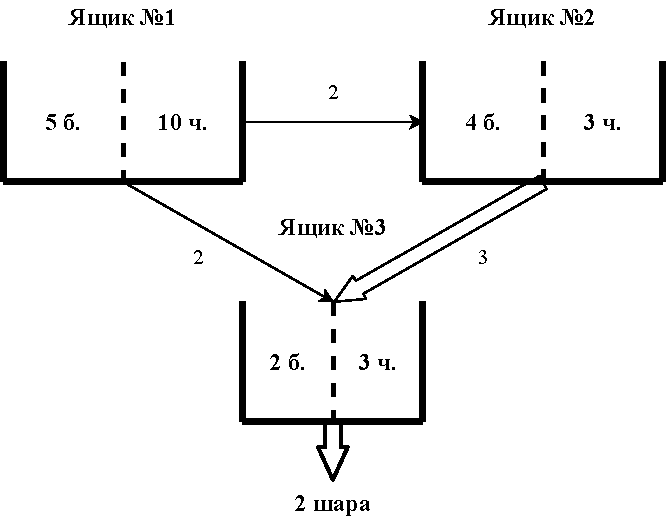
\includegraphics[scale=1]{./media/Homework-07-03-20_1.pdf}}
\end{figure}

\begin{enumerate}
	\item [а)] Определить вероятность, что из 3-его ящика вытащили шары одинаково цвета.
	\item [б)] Вытащили шары одного цвета, определить вероятность, что они изначально из одного ящика.
\end{enumerate}

\textit{Решение:}

\begin{enumerate}
	\item[а)] События $A_i, 0 \le i \le 2$ - из 1-ого ящика в 3-ий переложили $i$ белых и $2-i$ чёрных шаров образуют ПГС. Всего возможных вариантов данного действия: $C_{15}^2 = 105$.
	
	События $B_j, 0 \le j \le 2$ - из 1-го ящика во 2-й переложили $j$ белых и $2-j$ чёрных шаров.
	
	Построим таблицу условных вероятностей для каждого $B_j$-ого. Всего вариантов данного события (учитывая, что два уже вытащены из 1-го ящика): $C_{13}^2 = 78$. Если, например, из 1-го ящика в 3-й переложили 1 белый и 1 чёрный, то в 1-м ящике осталось 4 белых и 9 черных.
	
	\begin{table}[h]
		\centering\makegapedcells
		\begin{tabular}{|c|c|c|c|}
			\hline
			$i$          & 0                                                      & 1                                                       & 2                                                       \\ \hline
			$P(A_i)$     & $\frac{C_5^0 \cdot C_{10}^2}{C_{15}^2} = \frac{3}{7}$  & $\frac{C_5^1 \cdot C_{10}^1}{C_{15}^2} = \frac{10}{21}$ & $\frac{C_5^2 \cdot C_{10}^0}{C_{15}^2} = \frac{2}{21}$  \\ \hline
			$P(B_0|A_i)$ & $\frac{C_5^0 \cdot C_{8}^2}{C_{13}^2} = \frac{14}{39}$ & $\frac{C_4^0 \cdot C_{9}^2}{C_{13}^2} = \frac{6}{13}$   & $\frac{C_3^0 \cdot C_{10}^2}{C_{13}^2} = \frac{15}{26}$ \\ \hline
			$P(B_1|A_i)$ & $\frac{C_5^1 \cdot C_{8}^1}{C_{13}^2} = \frac{20}{39}$ & $\frac{C_4^1 \cdot C_{9}^1}{C_{13}^2} = \frac{6}{13}$   & $\frac{C_3^1 \cdot C_{10}^1}{C_{13}^2} = \frac{5}{13}$  \\ \hline
			$P(B_2|A_i)$ & $\frac{C_5^2 \cdot C_{8}^0}{C_{13}^2} = \frac{5}{39}$  & $\frac{C_4^2 \cdot C_{9}^0}{C_{13}^2} = \frac{1}{13}$   & $\frac{C_3^2 \cdot C_{10}^0}{C_{13}^2} = \frac{1}{26}$  \\ \hline
		\end{tabular}
	\end{table}
	
	По формуле ПГС найдём вероятности $P(B_0), P(B_1), P(B_2)$:
	
	\[ P(B_0) = \sum_{i=0}^{2} P(B_0|A_i) \cdot P(A_i) = \dfrac{3}{7} \]
	\[ P(B_1) = \sum_{i=0}^{2} P(B_1|A_i) \cdot P(A_i) = \dfrac{10}{21} \]
	\[ P(B_2) = \sum_{i=0}^{2} P(B_2|A_i) \cdot P(A_i) = \dfrac{2}{21} \]
	
	Видно, что вероятности $B_0, B_1, B_2$ также образуют ПГС.
	
	События $C_k, k=0,1,2,3$ - из 2-го ящика в 3-й переложили $k$ белых и $3-k$ чёрных шаров.
	
	\begin{table}[h]
		\centering\makegapedcells
		\begin{tabular}{|c|c|c|c|}
			\hline
			$B_i$        & $B_0$                                             & $B_1$                                             & $B_2$                                             \\ \hline
			$P(B_i)$     & $\frac{3}{7}$                                     & $\frac{10}{21}$                                   & $\frac{2}{21}$                                    \\ \hline
			$P(C_0|B_i)$ & $\frac{C_4^0 \cdot C_5^3}{C_9^3} = \frac{5}{42}$  & $\frac{C_5^0 \cdot C_4^3}{C_9^3} = \frac{1}{21}$  & $\frac{C_6^0 \cdot C_3^3}{C_9^3} = \frac{1}{84}$  \\ \hline
			$P(C_1|B_i)$ & $\frac{C_4^1 \cdot C_5^2}{C_9^3} = \frac{10}{21}$ & $\frac{C_5^1 \cdot C_4^2}{C_9^3} = \frac{5}{14}$  & $\frac{C_6^1 \cdot C_3^2}{C_9^3} = \frac{3}{14}$  \\ \hline
			$P(C_2|B_i)$ & $\frac{C_4^2 \cdot C_5^1}{C_9^3} = \frac{5}{14}$  & $\frac{C_5^2 \cdot C_4^1}{C_9^3} = \frac{10}{21}$ & $\frac{C_6^2 \cdot C_3^1}{C_9^3} = \frac{15}{28}$ \\ \hline
			$P(C_3|B_i)$ & $\frac{C_4^3 \cdot C_5^0}{C_9^3} = \frac{1}{21}$  & $\frac{C_5^3 \cdot C_4^0}{C_9^3} = \frac{5}{42}$  & $\frac{C_6^3 \cdot C_3^0}{C_9^3} = \frac{5}{21}$  \\ \hline
		\end{tabular}
	\end{table}
	
	Событие $D_l$ – в 3-й ящик попало $l$ белых и $5-l$ чёрных (из 1-го и 2-го ящика).
	
	\begin{table}[h]
		\centering\makegapedcells
		\begin{tabular}{|c|c|c|c|c|c|c|}
			\hline
			$l$                & 0            & 1                                                                      & 2                                                                                        & 3                                                                                        & 4                                                                      & 5            \\ \hline
			Комбинация событий & $(C_0, A_0)$ & \begin{tabular}[c]{@{}c@{}}$(C_1, A_0)$\\ \\ $(C_0, A_1)$\end{tabular} & \begin{tabular}[c]{@{}c@{}}$(C_2, A_0)$\\ \\ $(C_1, A_1)$\\ \\ $(C_0, A_2)$\end{tabular} & \begin{tabular}[c]{@{}c@{}}$(C_3, A_0)$\\ \\ $(C_2, A_1)$\\ \\ $(C_1, A_2)$\end{tabular} & \begin{tabular}[c]{@{}c@{}}$(C_3, A_1)$\\ \\ $(C_2, A_2)$\end{tabular} & $(C_3, A_2)$ \\ \hline
		\end{tabular}
	\end{table}
	
	\[ P(D_0) = P(C_0) \cdot P(A_0) = \dfrac{11}{147} \cdot \dfrac{3}{7} = \dfrac{11}{343} \]
	\[ P(D_1) = P(C_1) \cdot P(A_0) + P(C_0) \cdot P(A_1) = \dfrac{632}{3087} \]
	\[ P(D_2) = P(C_2) \cdot P(A_0) + P(C_1) \cdot P(A_1) + P(C_0) \cdot P(A_2) = \dfrac{1172}{3087} \]
	\[ P(D_3) = P(C_3) \cdot P(A_0) + P(C_2) \cdot P(A_1) + P(C_1) \cdot P(A_2) = \dfrac{892}{3087} \]
	\[ P(D_4) = P(C_3) \cdot P(A_1) + P(C_2) \cdot P(A_2) = \dfrac{820}{9261} \]
	\[ P(D_5) = P(C_3) \cdot P(A_2) = \dfrac{88}{9261} \]
	
	\[ \sum_{i=0}^{5} P(D_i) = 1 \Rightarrow \text{ события образуют ПГС} \]
	
	В результате в 3-ем ящике 10 шаров.
	
	Событие $E$ - из 3-го ящика достали \textbf{белый} шар.
	
	\begin{table}[H]
		\centering\makegapedcells
		\begin{tabular}{|c|c|c|c|c|c|c|}
			\hline
			$i$        & 0              & 1              & 2              & 3              & 4              & 5              \\ \hline
			$P(D_i)$   & 0.032          & 0.204          & 0.379          & 0.2855         & 0.0885         & 0.0095         \\ \hline
			$P(E|D_i)$ & $\frac{2}{10}$ & $\frac{3}{10}$ & $\frac{4}{10}$ & $\frac{5}{10}$ & $\frac{6}{10}$ & $\frac{7}{10}$ \\ \hline
		\end{tabular}
	\end{table}
	
	\[ P(E_1) = \sum_{i=0}^{5} P(D_i)P(E|D_i) = \dfrac{19631}{46305} \]
	
	Вероятность вытащить 2-ой белый шар будет равна:
	
	\begin{table}[H]
		\centering\makegapedcells
		\begin{tabular}{|c|c|c|c|c|c|c|}
			\hline
			$i$        & 0              & 1              & 2              & 3              & 4              & 5              \\ \hline
			$P(D_i)$   & 0.032          & 0.204          & 0.379          & 0.2855         & 0.0885         & 0.0095         \\ \hline
			$P(E|D_i)$ & $\frac{1}{9}$ & $\frac{2}{9}$ & $\frac{3}{9}$ & $\frac{4}{9}$ & $\frac{5}{9}$ & $\frac{6}{9}$ \\ \hline
		\end{tabular}
	\end{table}
	
	\[ P(E_2) = \sum_{i=0}^{5} P(D_i)P(E|D_i) = \dfrac{29969}{83349} \]
	
	Событие $N$ - достали два белых шара подряд:
	\[ P(N) = P(E_1) \cdot P(E_2) = \dfrac{588321439}{3859475445} \approx 0.152436 \]
	
	Событие $G$ - из 3-го ящика достали \textbf{чёрный} шар.
	
	\begin{table}[H]
		\centering\makegapedcells
		\begin{tabular}{|c|c|c|c|c|c|c|}
			\hline
			$i$        & 0              & 1              & 2              & 3              & 4              & 5              \\ \hline
			$P(D_i)$   & 0.032          & 0.204          & 0.379          & 0.2855         & 0.0885         & 0.0095         \\ \hline
			$P(G|D_i)$ & $\frac{3}{10}$ & $\frac{4}{10}$ & $\frac{5}{10}$ & $\frac{6}{10}$ & $\frac{7}{10}$ & $\frac{8}{10}$ \\ \hline
		\end{tabular}
	\end{table}
	
	\[ P(G_1) = \sum_{i=0}^{5} P(D_i)P(G|D_i) = \dfrac{1079}{2058} \]
	
	Вероятность вытащить 2-ой чёрный шар будет равна:
	
	\begin{table}[H]
		\centering\makegapedcells
		\begin{tabular}{|c|c|c|c|c|c|c|}
			\hline
			$i$        & 0              & 1              & 2              & 3              & 4              & 5              \\ \hline
			$P(D_i)$   & 0.032          & 0.204          & 0.379          & 0.2855         & 0.0885         & 0.0095         \\ \hline
			$P(G|D_i)$ & $\frac{2}{9}$ & $\frac{3}{9}$ & $\frac{4}{9}$ & $\frac{5}{9}$ & $\frac{6}{9}$ & $\frac{7}{9}$ \\ \hline
		\end{tabular}
	\end{table}
	
	\[ P(G_2) = \sum_{i=0}^{5} P(D_i)P(G|D_i) = \dfrac{39262}{83349} \]
	
	Событие $M$ - достали два чёрных шара подряд:
	\[ P(M) = G_1 \cdot G_2 = \dfrac{21181846}{85766121} \approx 0.246972 \]
	
	Событие $W$ - достали два шара одного цвета подряд, тогда:
	\[ P(W) = P(N) + P(M) = \dfrac{588321439}{3859475445} + \dfrac{21181846}{85766121} = \dfrac{15415044644}{3859475445} \approx 0.399408 \]
	
	\item[б)] 
\end{enumerate}

\newpage










\subsection*{Задача 3.}

Белые и чёрные шары распределены по ящикам следующим образом:

\begin{figure}[H]
	\center{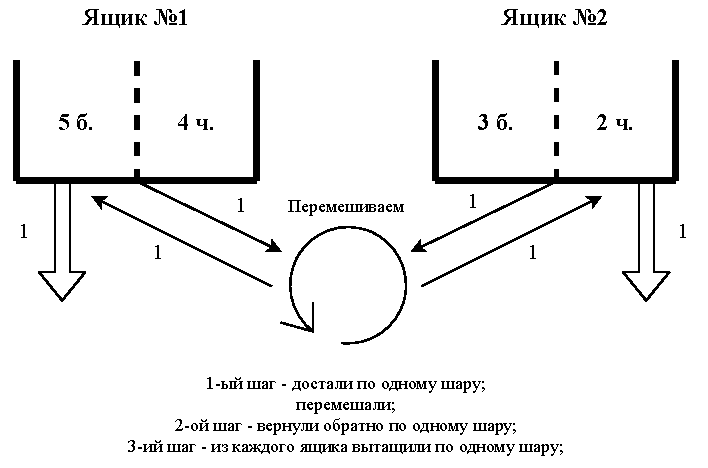
\includegraphics[scale=1]{./media/Homework-07-03-20_2.pdf}}
\end{figure}

\begin{enumerate}
	\item [а)] Определить вероятность, что шары, вытащенные на 3-ем шаге, одного цвета.
	\item [б)] Определить вероятность, что цветовой состав ящиков до вытаскивания на 3-ем шаге, не изменился.
\end{enumerate}

\textit{Решение:}

\begin{enumerate}
	\item[а)] Рассмотрим 1-ый шаг с перемешиванием. По условию задачи мы не различаем шары между собой, как следствие, если мы вытащили шары одного цвета (ББ или ЧЧ), то ситуация не поменяется. Событие $O$ - достали только белые, $L$ - достали только чёрные.
	\[ P(O) = \dfrac{5}{9} \cdot \dfrac{3}{5} = \dfrac{1}{3} \]
	\[ P(L) = \dfrac{4}{9} \cdot \dfrac{2}{5} = \dfrac{8}{45} \]
	
	Рассмотрим события, когда достали БЧ и ЧБ. Событие $W$ - достали БЧ, событие $B$ - ЧБ.
	\[ P(W) = \dfrac{5}{9} \cdot \dfrac{2}{5} = \dfrac{2}{9} \]
	\[ P(B) = \dfrac{4}{9} \cdot \dfrac{3}{5} = \dfrac{4}{15} \]
	 
	 Вероятность, что данные шары поменялись местами $P(C) = \dfrac{1}{2}$, т.е. вероятность, что в ящик вернётся не тот цвет, что оттуда брали.
	 
	 Событие $R$ - вытащили два одинаковых шара.
	 
	 \[ P(RO) = \dfrac{1}{3} \cdot \left( \left( \dfrac{5}{9} \cdot \dfrac{3}{5} \right) + \left( \dfrac{4}{9} \cdot \dfrac{2}{5} \right) \right) = \dfrac{23}{45} \cdot \dfrac{1}{3} = \dfrac{23}{135} \]
	 
	 \[ P(RL) = \dfrac{8}{45} \cdot \left( \left( \dfrac{5}{9} \cdot \dfrac{3}{5} \right) + \left( \dfrac{4}{9} \cdot \dfrac{2}{5} \right) \right) = \dfrac{23}{45} \cdot \dfrac{8}{45} = \dfrac{184}{2025} \]
	 
	 \[
	 P(RW) = +
		 \left.
			 \begin{array}{cc}
				 \dfrac{1}{2} \cdot \left( \left( \dfrac{5}{9} \cdot \dfrac{3}{5} \right) + \left( \dfrac{4}{9} \cdot \dfrac{2}{5} \right) \right) & = \dfrac{23}{90} \\
				 \dfrac{1}{2} \cdot \left( \left( \dfrac{4}{9} \cdot \dfrac{4}{5} \right) + \left( \dfrac{5}{9} \cdot \dfrac{1}{5} \right) \right) & = \dfrac{7}{30} \\
			 \end{array}
		 \right\}
	 \cdot \dfrac{2}{9} = \dfrac{22}{45} \cdot \dfrac{2}{9}  = \dfrac{44}{405}
	 \]
	 
	 \[
	 P(RB) = +
	 	\left.
		 	\begin{array}{cc}
			 	\dfrac{1}{2} \cdot \left( \left( \dfrac{5}{9} \cdot \dfrac{3}{5} \right) + \left( \dfrac{4}{9} \cdot \dfrac{2}{5} \right) \right) & = \dfrac{23}{90} \\
			 	\dfrac{1}{2} \cdot \left( \left( \dfrac{6}{9} \cdot \dfrac{2}{5} \right) + \left( \dfrac{3}{9} \cdot \dfrac{3}{5} \right) \right) & = \dfrac{7}{30} \\
		 	\end{array}
		 	\right\}
	 	\cdot \dfrac{4}{15} = \dfrac{22}{45} \cdot \dfrac{4}{15}  = \dfrac{88}{675}
	 \]
	 
	 \[ P(R) = \dfrac{23}{135} + \dfrac{184}{2025} + \dfrac{44}{405} + \dfrac{88}{675} = \dfrac{1013}{2025} \]
	 
	 \item[б)] Складываем вероятности из того, что либо бы брали шары одинаково цвета, либо с вероятностью $\frac{1}{2}$ они не поменялись местами, когда взяли разного:
	 
	 \[ \dfrac{1}{3} + \dfrac{8}{45} + \dfrac{1}{2} \cdot \dfrac{2}{9} + \dfrac{1}{2} \cdot \dfrac{4}{15} = \dfrac{34}{45} \]
\end{enumerate}

\newpage










\subsection*{Задача 4.}

\begin{figure}[H]
	\center{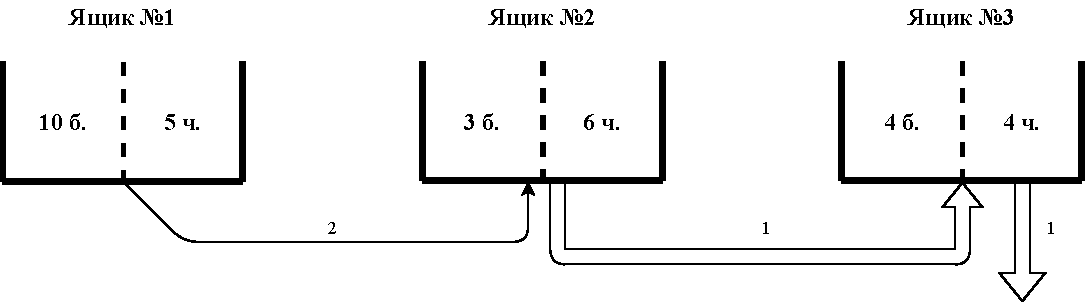
\includegraphics[scale=1]{./media/Homework-07-03-20_3.pdf}}
\end{figure}

\begin{enumerate}
	\item [а)] Определить вероятность, что из 3-его ящика достали белый шар.
	\item [б)] Из 3-его ящика вытащен белый, найти вероятность, что следующий шар, доставаемый из 3-его тоже белый.
\end{enumerate}

\textit{Решение:}

\begin{enumerate}
	\item[а)] Событие $A$ - из 3-его ящика достали белый шар.
	
	Событие $H_i$ - шар, вытащенный из 3-его ящика, изначально находился в $i$-ом ящике.
	
	\begin{table}[h]
		\centering\makegapedcells
		\begin{tabular}{|c|c|c|c|}
			\hline
			$i$        & 1                           & 2                         & 3                         \\ \hline
			$P(H_i)$   & $?$                         & $?$                       & $\frac{8}{9}$             \\ \hline
			$P(A|H_i)$ & $\frac{10}{15}=\frac{2}{3}$ & $\frac{3}{9}=\frac{1}{3}$ & $\frac{4}{8}=\frac{1}{2}$ \\ \hline
		\end{tabular}
	\end{table}

	Событие $B_j$ - вытащенный из 3-его ящика шар, попал туда из $j$-ого ящика одним текущим перекладыванием.
	
	\begin{table}[h]
		\centering\makegapedcells
		\begin{tabular}{|c|c|c|c|}
			\hline
			$i$        & 1 & 2             & 3             \\ \hline
			$P(B_i)$   & 0 & $\frac{1}{9}$ & $\frac{8}{9}$ \\ \hline
			$P(A|B_i)$ & ? & ?             & $\frac{1}{2}$ \\ \hline
		\end{tabular}
	\end{table}


	$P(H_1|B_2) = \dfrac{P(H_1B_2)}{P(B_2)}= \dfrac{2}{3 + 6 + 2} = \dfrac{2}{11}$ - вероятность вытащить шар, изначально находившийся в 1-ом ящике из 2-ого.
	
	$P(H_2|B_2) = \dfrac{9}{3 + 6 + 2} = \dfrac{9}{11}$
	
	Если шар был изначально в 3-м ящике, то он не был переложен в него (и наоборот), т.е. $H_3=B_3$. Если же шар изначально был в 1-м, то он был переложен из 1-го во 2-й, а из 2-ого в 3-й.
	\[ P(H_1) = P(H_1B_2) = P(H_1|B_2) \cdot P(B_2) = \dfrac{2}{11} \cdot \dfrac{1}{9} = \dfrac{2}{99} \]
	
	Если шар изначально был в 2-м ящике, то он не был переложен во 2-й из 1-ого, но был переложен из 2-ого в 3-й.
	\[ P(H_2) = P(H_2B_2) = P(H_2|B_2) \cdot P(B_2) = \dfrac{9}{11} \cdot \dfrac{1}{9} = \dfrac{1}{11} \]
	
	\begin{table}[h]
		\centering\makegapedcells
		\begin{tabular}{|c|c|c|c|}
			\hline
			$i$        & 1              & 2              & 3             \\ \hline
			$P(H_i)$   & $\frac{2}{99}$ & $\frac{1}{11}$ & $\frac{8}{9}$ \\ \hline
			$P(A|H_i)$ & $\frac{2}{3}$  & $\frac{1}{3}$  & $\frac{1}{2}$ \\ \hline
		\end{tabular}
	\end{table}

	\[ P(A) = \sum_{i=1}^3 P(A|H_i)P(H_i) = \dfrac{145}{297} \approx 0.488215 \]
	
	\item[б)] Вероятность, что следующий вытащенный шар также окажется белым.
	
	\begin{align*}
		\fbox{%
			\parbox{8cm}{%
				1-ый шар, который мы достали из 3-его ящика и который изначально находился в 1-ом или 2-ом ящиках, исключает возможность получения из них же 2-ого шара, который достают из 3-его ящика}%
		}
	\end{align*}
	
	По формуле Байеса:
	\[ P(H_3|A) = \dfrac{P(A|H_3)P(H_3)}{P(A)} = \dfrac{\frac{1}{2} \cdot \frac{8}{9}}{\frac{145}{297}} = \dfrac{132}{145} \]
	\[ P(H_2|A) = \dfrac{P(A|H_2)P(H_2)}{P(A)} = \dfrac{\frac{1}{3} \cdot \frac{1}{11}}{\frac{145}{297}} = \dfrac{9}{145} \]
	\[ P(H_1|A) = \dfrac{P(A|H_1)P(H_1)}{P(A)} = \dfrac{\frac{2}{3} \cdot \frac{2}{99}}{\frac{145}{297}} = \dfrac{4}{145} \]
	
	Событие $C$ - следующий вытащенный шар также оказался белым.
	
	Событие $G_k$ - вытащенный из 3-его ящика второй шар, изначально находился в $k$-ом ящике.
	
	Если мы достали шар, изначально находившийся в 1-м или 2-м ящике, то 2-ой шар обязан быть из 3-его, т.к. в него положили только один шар из другого ящика.
	
	Если же первым шагом мы достали шар, изначально находившийся в 3-ем ящике, то 2-м может быть шар, пришедший из всех 3-х ящиков.
	
	Т.к. по условию задачи выполнение события $A$ является обязательным, то в рамках решения данной задачи можно считать, что:
	\[ P(H_3) = \dfrac{132}{145}, P(H_2) = \dfrac{9}{145}, P(H_1) = \dfrac{4}{145} \]
	
	\begin{table}[h]
		\centering\makegapedcells
		\begin{tabular}{|c|c|c|c|}
			\hline
			$i$          & 1               & 2               & 3                 \\ \hline
			$P(H_i)$     & $\frac{4}{145}$ & $\frac{9}{145}$ & $\frac{132}{145}$ \\ \hline
			$P(G_1|H_i)$ & 0               & 0               & $?$               \\ \hline
			$P(G_2|H_i)$ & 0               & 0               & $?$               \\ \hline
			$P(G_3|H_i)$ & 1               & 1               & $\frac{7}{8}$     \\ \hline
		\end{tabular}
	\end{table}

	Событие $F_l$ - 2-ой вытащенный из 3-его ящика шар был переложен туда из $l$-ого ящика.
	
	\begin{table}[h]
		\centering\makegapedcells
		\begin{tabular}{|c|c|c|c|}
			\hline
			$i$          & 1 & 2             & 3             \\ \hline
			$P(F_l|H_3)$ & 0 & $\frac{1}{8}$ & $\frac{7}{8}$ \\ \hline
		\end{tabular}
	\end{table}

	$P(G_1|F_2H_3) = \dfrac{2}{11}$ - вероятность, что 2-ой шар, который достали из 3-его ящика, был изначально в 1-ом, при условии, что 1-м шаром из 3-его ящика достали шар, который там и был, а 2-ой совершил путь $1\to2\to3$.
	
	$P(G_2|F_2H_3) = \dfrac{9}{11}$ -  вероятность, что 2-ой шар, который достали из 3-его ящика, был изначально в 2-ом, при условии, что 1-м шаром из 3-его ящика достали шар, который там и был, а 2-ой совершил путь $2\to3$.
	
	Если шар был изначально в 3-м, то он не был переложен (и наоборот, то есть $D_3=F_3$).
	
	Если шар изначально был в 1-м, то он был переложен из 1-го во 2-й, а из 2-го в 3-й, т.е.
	\[ P(G_1H_3) = P(G_1F_2H_3) = P(G_1|F_2H_3) \cdot P(F_2|H_3) \cdot P(H_3) = \dfrac{2}{11} \cdot \dfrac{1}{8} \cdot \dfrac{132}{145} = \dfrac{3}{145} \]
	
	Если шар изначально был в 2-м, то он не был переложен из 1-го во 2-й, но совершил путь из 2-ого в 3-ий, т.е.
	\[ P(G_2H_3) = P(G_2F_2H_3) = P(G_2|F_2H_3) \cdot P(F_2|H_3) \cdot P(H_3) = \dfrac{9}{11} \cdot \dfrac{1}{8} \cdot \dfrac{132}{145} = \dfrac{27}{290} \]
	
	Если шар изначально был в 3-ем ящике, то его никуда не перекладывали и зависимости от перемещений нет, т.е
	\[ P(G_3H_3) = P(G_3|H_3) \cdot P(H_3) = \dfrac{7}{8} \cdot \dfrac{132}{145} = \dfrac{231}{290} \]
	
	Из приведённой выше таблицы видно, что:
	\[ P(G_1H_2) = P(G_2H_2) = 0 \text{ (единств. перешедший шар достали)}\]
	\[ P(G_3H_2) = P(H_2) = \dfrac{9}{145} \text{ (единств. перешедший шар достали, а значит } G_3 = 1 \text{)} \]
	
	\[ P(G_1H_1) = P(G_2H_1) = 0 \]
	\[ P(G_3H_1) = P(H_1) = \dfrac{4}{145} \]
	
	\[ P(G_1) = \underbrace{P(G_1H_1)}_{=0} + \underbrace{P(G_1H_2)}_{=0} + P(G_1H_3) = \dfrac{3}{145} \]
	\[ P(G_2) = \underbrace{P(G_2H_1)}_{=0} + \underbrace{P(G_2H_2)}_{=0} + P(G_2H_3) = \dfrac{27}{290} \]
	\[ P(G_3) = P(G_3H_1) + P(G_3H_2) + P(G_3H_3) = \dfrac{4}{145} + \dfrac{9}{145} + \dfrac{231}{290} = \dfrac{257}{290} \]
	
	\[ P(G_1) + P(G_2) + P(G_3) = 1 \Rightarrow \text{ образуют ПГС} \]
	
	На вероятность достать 2-м белый шар также будет влиять их начальное перемещение по ящикам, в случае, если 1-ый и 2-ой шары, которые мы достаём из 3-его ящика изначально были в одном.
	
	Рассмотрим зависимость вероятности события $C$ от того, откуда пришёл вытащенный на 1-ом этапе шар:
	
	\begin{table}[h]
		\centering\makegapedcells
		\begin{tabular}{|c|c|c|c|c|c|}
			\hline
			$(i,j)$       & $(3,1)$         & $(3,2)$         & $(3,3)$           & $(2,3)$          & $(1,3)$         \\ \hline
			$P(G_iH_j)$   & $\frac{4}{145}$ & $\frac{9}{145}$ & $\frac{231}{290}$ & $\frac{27}{290}$ & $\frac{3}{145}$ \\ \hline
			$P(C|G_iH_j)$ & $\frac{1}{2}$   & $\frac{1}{2}$   & $\frac{3}{7}$     & $\frac{1}{3}$    & $\frac{2}{3}$   \\ \hline
		\end{tabular}
	\end{table}

	В результате:
	
	\[ P(C) = \sum P(G_iH_j) P(C|G_iH_j), i=3,3,3,2,1; j=1,2,3,3,3 \]
	\[ P(C) = \dfrac{25}{58} \approx 0.431034 \]
	
\end{enumerate}

\end{document} 